\documentclass[12pt, a4paper, oneside]{Thesis} % Paper size, default font size and one-sided paper
\usepackage{wrapfig}
\usepackage{lscape}
\usepackage{rotating}
\usepackage{graphicx}
\usepackage{caption}
\usepackage{amsmath}
\usepackage{paralist}
\usepackage{tasks}
\usepackage{amssymb}

\usepackage{lineno,hyperref}
\modulolinenumbers[5]

\usepackage[table,xcdraw]{xcolor}
\usepackage{amssymb}
\usepackage{upgreek}
\usepackage{graphicx}
\usepackage{array}
\usepackage{float}
\usepackage{placeins}
\usepackage{stackengine}
\usepackage{url}
\usepackage{numprint}
\usepackage{caption}
\usepackage{enumerate}

\usepackage{booktabs}  
\usepackage{siunitx}
%\usepackage[showframe=false]{geometry}
\usepackage{subfigure}
\usepackage[hashEnumerators,smartEllipses]{markdown}

\nprounddigits{3}
\newcolumntype{P}[1]{>{\centering\arraybackslash}p{#1}}
\newcolumntype{M}[1]{>{\centering\arraybackslash}m{#1}}

\setstackEOL{\#}
\setstackgap{L}{12pt}

\newenvironment{tightcenter}{%
  \setlength\topsep{0pt}
  \setlength\parskip{0pt}
  \begin{center}
}{%
  \end{center}
}

%\usepackage{subcaption} %incompatible with subfig
\graphicspath{{Pictures/}} % Specifies the directory where pictures are stored
\usepackage{natbib} % Use the natbib reference package - read up on this to edit the reference style; if you want text (e.g. Smith et al., 2012) for the in-text references (instead of numbers), remove 'numbers' v

\hypersetup{urlcolor=black, colorlinks=false} % Colors hyperlinks in blue - change to black if annoyingv`	

\thesistitle{A Thesis on Emotion Recognition using EEG Signals}
\supervisor{Professor Debasis Samanta}
\degree{Master of Technology}
\degreemajor{Computer Science \& Engineering}
\authors{Sayan Naskar}
\rollno{15CS30027}
\university{Indian Institute of Technology Kharagpur}
\department{Department of Computer Science \& Engineering}
\unisite{http://www.iitkgp.ac.in}
\depsite{http://www.cse.iitkgp.ac.in/}
\placeshrt{Kharagpur}
\placelng{Kharagpur - 721302, India}
\datesub{May 21, 2020}
\datesig{May 21, 2020}
\semsub{Spring Semester, 2019-20}
\keywords{Signal Processing, EEG Signals}
\coursecd{Project-II (CS57004) }

\title{\ttitle} % Defines the thesis title - don't touch this
\begin{document}
%\makeatletter
%\renewcommand*{\NAT@nmfmt}[1]{\textsc{#1}}
%\makeatother

% prints author names as small caps


\frontmatter % Use roman page numbering style (i, ii, iii, iv...) for the pre-content pages

\setstretch{1.6} % Line spacing of 1.6 (double line spacing)

% Define the page headers using the FancyHdr package and set up for one-sided printing
\fancyhead{} % Clears all page headers and footers
\rhead{\thepage} % Sets the right side header to show the page number
\lhead{} % Clears the left side page header

%\pagestyle{fancy} % Finally, use the "fancy" page style to implement the FancyHdr headers

\newcommand{\HRule}{\rule{\linewidth}{0.5mm}} % New command to make the lines in the title page

% PDF meta-data
\hypersetup{pdftitle={\ttitle}}
\hypersetup{pdfsubject=\subjectname}
\hypersetup{pdfauthor=\authornames}
\hypersetup{pdfkeywords=\keywordnames}

%----------------------------------------------------------------------------------------
%	TITLE PAGE
%----------------------------------------------------------------------------------------
\maketitle
%\titlepg % Add a gap in the Contents, for aesthetics

\clearpage % Start a new page

%----------------------------------------------------------------------------------------
%	DECLARATION PAGE
%	Your institution may give you a different text to place here
%----------------------------------------------------------------------------------------


\Declaration% Add a gap in the Contents, for aesthetics


%----------------------------------------------------------------------------------------
%	CERTIFICATE PAGE
%----------------------------------------------------------------------------------------

\addtotoc{Certificate} % Add the "Abstract" page entry to the Contents

\certificate{\addtocontents{toc}{} % Add a gap in the Contents, for aesthetics

\clearpage % Start a new page

%----------------------------------------------------------------------------------------
%	ABSTRACT PAGE
%----------------------------------------------------------------------------------------

\addtotoc{Abstract} % Add the "Abstract" page entry to the Contents

\abstract{\addtocontents{toc}{} % Add a gap in the Contents, for aesthetics

Enter content here. 
}

\clearpage % Start a new page



%----------------------------------------------------------------------------------------
%	ACKNOWLEDGEMENTS
%----------------------------------------------------------------------------------------

\setstretch{1.3} % Reset the line-spacing to 1.3 for body text (if it has changed)

\acknowledgements{\addtocontents{toc}{}%\vspace{1em}} % Add a gap in the Contents, for aesthetics

I would like to sincerely thank Prof. Debasis Samanta and Miss Sricheta Parui for their guidance.

}
\clearpage % Start a new page

%----------------------------------------------------------------------------------------
%	LIST OF CONTENTS/FIGURES/TABLES PAGES
%----------------------------------------------------------------------------------------

\pagestyle{fancy} % The page style headers have been "empty" all this time, now use the "fancy" headers as defined before to bring them back

\lhead{\emph{Contents}} % Set the left side page header to "Contents"
\tableofcontents % Write out the Table of Contents

\lhead{\emph{List of Figures}} % Set the left side page header to "List of Figures"
\listoffigures % Write out the List of Figures

\lhead{\emph{List of Tables}} % Set the left side page header to "List of Tables"
\listoftables % Write out the List of Tables

%----------------------------------------------------------------------------------------
%	ABBREVIATIONS
%----------------------------------------------------------------------------------------

\clearpage % Start a new page

\setstretch{1.5} % Set the line spacing to 1.5, this makes the following tables easier to read



%----------------------------------------------------------------------------------------
%	PHYSICAL CONSTANTS/OTHER DEFINITIONS
%----------------------------------------------------------------------------------------
%
%\clearpage % Start a new page
%
%\lhead{\emph{Physical Constants}} % Set the left side page header to "Physical Constants"
%
%\listofconstants{lrcl} % Include a list of Physical Constants (a four column table)
%{
%Speed of Light & $c$ & $=$ & $2.997\ 924\ 58\times10^{8}\ \mbox{ms}^{-\mbox{s}}$ (exact)\\
%% Constant Name & Symbol & = & Constant Value (with units) \\
%}

%----------------------------------------------------------------------------------------
%	SYMBOLS
%----------------------------------------------------------------------------------------



%----------------------------------------------------------------------------------------
%	DEDICATION
%----------------------------------------------------------------------------------------
%
%\setstretch{1.3} % Return the line spacing back to 1.3
%
%\pagestyle{empty} % Page style needs to be empty for this page
%
%\dedicatory{For/Dedicated to/To my\ldots} % Dedication text
%
%\addtocontents{toc}{\vspace{2em}} % Add a gap in the Contents, for aesthetics

%----------------------------------------------------------------------------------------
%	THESIS CONTENT - CHAPTERS
%----------------------------------------------------------------------------------------

\mainmatter % Begin numeric (1,2,3...) page numbering

\pagestyle{fancy} % Return the page headers back to the "fancy" style

% Include the chapters of the thesis as separate files from the Chapters folder
% Uncomment the lines as you write the chapters

% Chapter Template

\chapter{Introduction} % Main chapter title

\label{Chapter 1} % Change X to a consecutive number; for referencing this chapter elsewhere, use \ref{ChapterX}

\lhead{Chapter 1. \emph{Introduction}} % Change X to a consecutive number; this is for the header on each page - perhaps a shortened title

%----------------------------------------------------------------------------------------
%	SECTION 1
%----------------------------------------------------------------------------------------

\section{Problem Statement}
The brain is one of the most intricate, complex and fascinating elements of the universe. It allows us to remember past events, process every sensory impression, and project all our thoughts, memories and estimations into the future.

The topic of interest is Emotion Recognition and Estimation. If a machine can recognize the emotional state of the user, it will be possible to automate tasks taking into account the current emotional state of the user. There are several ways to recognize emotional states
\begin{enumerate}
\item Facial Expression using \emph{Camera}
\item Voice and Audio using \emph{Microphone}
\item Brain Activity Signals using \emph{BCI devices like EEG, MEG, PET, MRI}
\end{enumerate}

In the first semester of Master's Thesis, the goal was to explore Human Computer Interaction using Brain Computer Interface (HCI-BCI). The methodologies of collecting data about brain activity (Brain signals) and processing these signals to get rich features about the brain activity was studied. What is noise and artefact in the context of a particular experiment? How can the brain signal be processed to get enriched data? These were the questions asked and explored.

In the second and final semester, the goal was to explore solutions to the problem using machine learning models. 

\section{Brain Waves}
\begin{figure}[H]
\centering
\includegraphics[height=4cm]{Pictures/brainwavefrequencies.png}
\caption{Brain Wave Classification based on frequency}
\label{fig11}
\end{figure}

\section{Electroencephalography}

Electroencephalography (EEG) is a physiological monitoring method to record electrical activity of the brain. Electroencephalography records the electrical activity of the brain using electrodes placed on the scalp. Measuring electrical activity from the brain is useful because it reflects how the many different neurons in the brain network communicate with each other via electrical impulses.

\subsection{10-20 electrode system}
\begin{figure}[H]
\centering
\includegraphics[height=7cm]{Pictures/1020.png}
\caption{The 10-20 electrode system with 32 electrodes}
\label{fig12}
\end{figure}

In the 10-20 system, electrode names begin with one or two letters indicating the general brain region or lobes where the electrode is placed:

\bfseries \normalfont
\begin{tasks}[label-align=left, label-offset={0mm}, label-width={5mm}, item-indent={5mm}, label-format={\bfseries}, column-sep=10mm](4)
\task \textbf{Fp} Frontopolar
\task \textbf{F} Frontal
\task \textbf{C} Central
\task \textbf{P} Parietal
\task \textbf{O} Occipital
\task \textbf{T} Temporal
\end{tasks}

Each electrode name ends with a number or letter indicating the distance to the midline. Odd numbers are used in the left hemisphere, even numbers in the right hemisphere. Larger numbers indicate greater distances from the midline, while electrodes placed at the midline are labeled with a z for zero. For example, Cz is placed over midline central brain regions, Fp8 is placed over right fronto-polar brain regions, and T7 is placed over left temporal regions.
% Chapter Template

\chapter{Literature Survey} % Main chapter title

\label{Chapter2} % Change X to a consecutive number; for referencing this chapter elsewhere, use \ref{ChapterX}

\lhead{Chapter 2. \emph{Literature Survey}} % Change X to a consecutive number; this is for the header on each page - perhaps a shortened title

Some of the papers studied for references are:
\begin{itemize}
\item ``Mahnob-HCI-Tagging Database \emph{(Lichtenauer et. al., 2012)}''\cite{mahnobDataset}
\item ``Analysis of EEG signals and facial expressions for continuous emotion detection \emph{(Soleymani et. al., 2015)}''\cite{mahnobEmo}
\item ``Emotion Classification in Arousal Valence Model using MAHNOB-HCI Database \emph{(Wiem et. al., 2017)} \cite''{wiem}
\item ``Selection of the Most Relevant Physiological Features for Classifying Emotion \emph{(Godin et. al., 2015)}''\cite{sel}

After reading these past journals, conference papers and theses, I arrived to these conclusions:
\begin{enumerate}
    \item Human Computer Interaction is a complex topic, and it requires Medical, Mathematical (Signal Processing and Statistical) Knowledge.
    \item There is no way to remove noise and artefacts from collected signal once it has been collected. Hence, while collecting data, you need to be as accurate and careful as possible.
    \item Multiple organs interfere with brain signals and hence are a source of noise to the EEG signals. Subtracting or negating the noise provided by these organs is not always possible, and if possible, it isn't quite precise. Some examples are 
    \begin{enumerate}
        \item Heart activities or ECG signals
        \item Eye Activity, i.e., rotation and focus of the eyes.
        \item Loss of focus or attention by the participant. In this case, the brain activities are not a result of the desired external stimuli , but by wither some internal stimuli or other undesired external stimuli.
    \end{enumerate}
    \item There aren't many clean datasets available freely.
    \item The accuracy varies a lot according to the methodology and dataset used.
    \item Given the brain activity reading, we can segment it into chunks of data of smaller durations, and use the label (ground truth values) on the parent data as the label of all the chunks.
\end{enumerate}
\end{itemize}



% I attempted doing the project using MNE tools in python. I faced quite a bit of issues, and switched to MATLAB for preprocessing.

% Here is the analysis of the signal processing steps, and the reason behind doing the steps:
% \begin{itemize}
% \item Collect High Density EEG Data: The data is collected at a high sampling rate. This is done because data can be down-sampled without loss, however it can't be up-sampled correctly.
% The data collected should be as much free from noise as possible.
% \item The EEG event structure contains records of the experimental events that occurred while the data was being recorded. This can be anything from mouse clicks, video playing on, off, etc.
% \item The data is referenced to either some electrode, or the average reference is taken for each electrode.
% \item The EEG data is down-sampled to reduce the input size. An overwhelming input size may cause over-fitting.
% \item Since the experiment type is Emotion Elicitation, we remove the frequencies which correspond to low activity mental state. Typically, the frequencies below 0.1Hz are removed.
% \item The line noise is removed. Sharp peaks or outliers are smoothed. This is done using a tool called CleanLine.
% \item The required channels are picked and the bad and the channels not required are rejected.
% \item The EEG Epochs corresponding to desired events are chosen.
% \item Finally we run ICA to get the independent components from the electrode signals. ICA finds directions in the feature space corresponding to projections with high non-Gaussianity. We thus obtain a decomposition into independent components, and the artifact’s contribution is localized in only a small number of components. These components have to be correctly identified and removed.
% \end{itemize}

% \section{Difficulties faced}
% \begin{itemize}
% \item Preprocessing the data using MNE python was challenging; there were plenty to methods in the library, but there was no concrete pipeline-based approach to data preprocessing unlike in EEGLab tutorials.
% \item I switched to EEGLab later. However scripting in MATLAB was unfamiliar to me. The way to do the same preprocessing for every EEG file was unknown.
% \item MAHNOB HCI contains 30 seconds of non-event data before and after the actual EEG Signal containing events. Removing these using EEGLAB was difficult as I could find no way to reference index with respect to the end time of the EEG file.
% \item Slicing the EEG data between [30s:-30s] was easy in MNE but data could only be exported as “FIF” file, which was unreadable by EEGLab.
% \end{itemize}

% \section{Experimental Results}
% \begin{itemize}
% \item As of now, I could only process individual EEG file and export the down-sampled, filtered EEG file which contained little noise.
% \item I performed Independent Component Analysis on the data to get the almost uncorrelated dimensions.
% \item I converted the data from time domain to frequency domain and applied PSD to get the four types of Brain Waves : delta, theta, alpha, beta
% \end{itemize}

% \begin{figure}[H]
% \centering
% \includegraphics[height=7cm]{Pictures/psd01.jpg}
% \caption{PSD Before Preprocessing}
% \label{fig24}
% \end{figure}
% \begin{figure}[H]
% \centering
% \includegraphics[height=6cm]{Pictures/psd02.jpg}
% \caption{PSD After Preprocessing}
% \label{fig25}
% \end{figure}

% \begin{figure}[H]
% \centering
% \includegraphics[height=6cm]{Pictures/tm02.jpg}
% \caption{Amplitude vs Time Before Preprocessing}
% \label{fig26}
% \end{figure}
% \begin{figure}[H]
% \centering
% \includegraphics[height=6cm]{Pictures/tm01.jpg}
% \caption{Amplitude vs Time After Preprocessing}
% \label{fig27}
% \end{figure}

% \section{Future Work}
% In the future, exploring novel methods of feature extraction and fitting these into classifying models such as regression models, SVM, XGBoost etc. will be the focus. I also plan to trying out analysis and experiments in Python, because being a veteran programming language, projects and code in python can easily be extended and reproduced.
 
% Chapter Template

\chapter{Proposed Methodology} % Main chapter title

\label{Chapter3} % Change X to a consecutive number; for referencing this chapter elsewhere, use \ref{ChapterX}

\lhead{Chapter 3. \emph{Proposed Methodology}} % Change X to a consecutive number; this is for the header on each page - perhaps a shortened title

The proposal of the method used to recognise a sample EEG signal is as follows:
\begin{enumerate}
    \item We select a dataset containing (EEG signal, Emotion) data pair. In this project, MAHNOB-HCI Dataset is used.
    \item The EEG files from the selected dataset is first cropped to extract the brain activity of the time only when the external stimuli is applied.
    \item The cropped data is divided into chunks of equal size.
    \item Each channel of every chunk is processed by multiple functions, where each function outputs one or more values, corresponding to a feature.
    \item All the features of a single channel are collected. The respective features are averaged, if desired, else all of them are appended.
    \item The feature vector thus obtained is supplied as data to the ML model, which is trained to for this supervised learning task.
    \item For predicting the emotion from an external EEG signal, it needs to be passed through the same pipeline, and it might give more than one output values (which depends on the size of the test data). The output of the complete EEG reading can be interpreted by any reduction method, such as mean, median and mode.
\end{enumerate} 
% Chapter Template

\chapter{Dataset Used: MAHNOB-HCI Tagging Database} % Main chapter title

\label{Chapter4} % Change X to a consecutive number; for referencing this chapter elsewhere, use \ref{ChapterX}

\lhead{Chapter 4. \emph{Dataset Used: MAHNOB-HCI Tagging Database}} % Change X to a consecutive number; this is for the header on each page - perhaps a shortened title

The components of the database are as shown in the diagram below.

\begin{figure}[H]
\centering
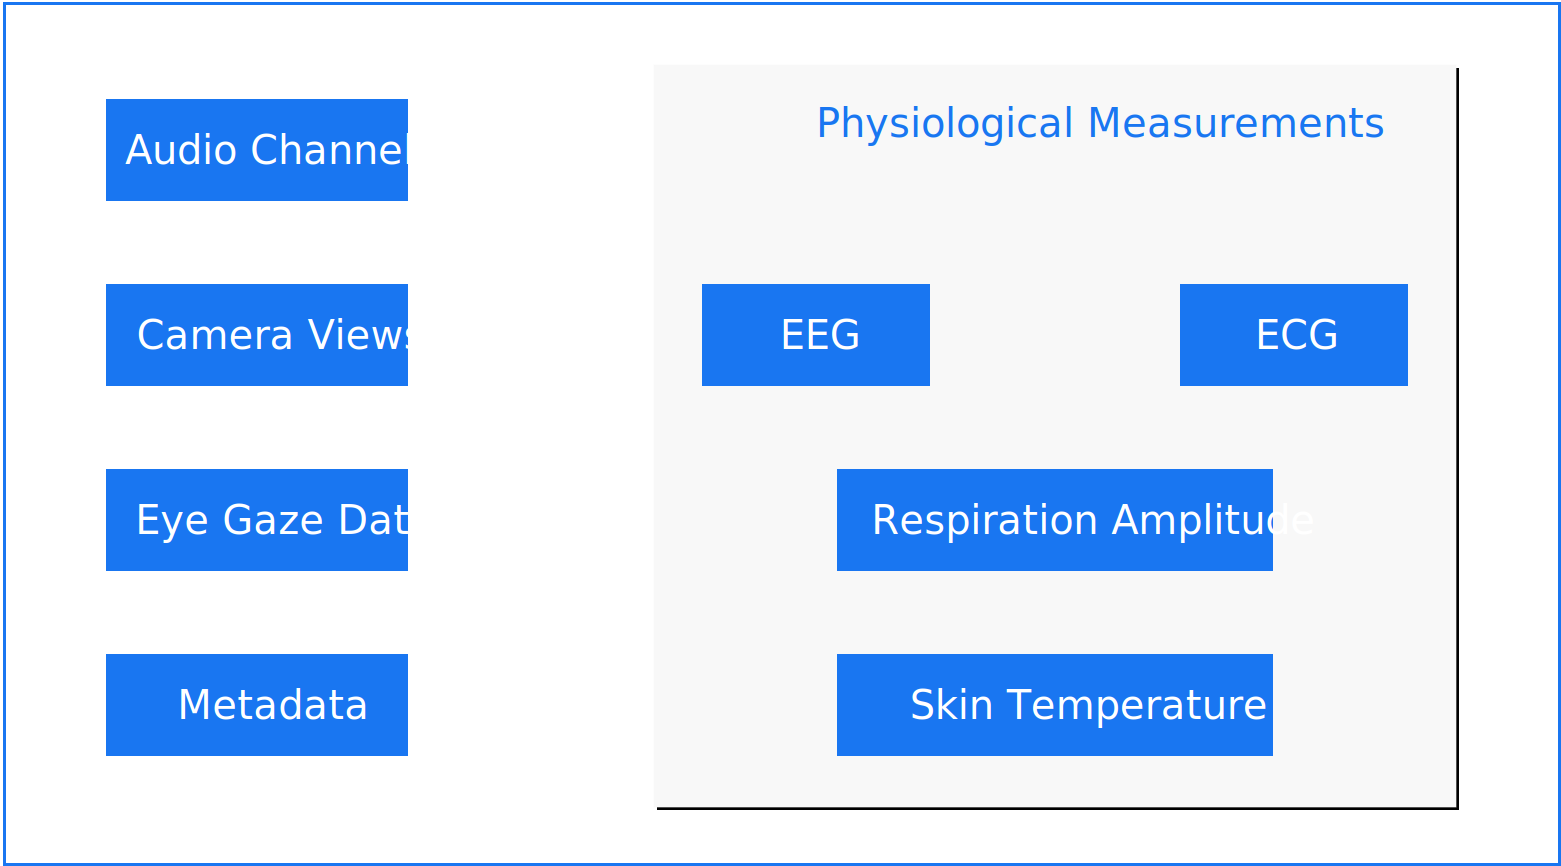
\includegraphics[height=7cm]{Figures/dataset.png}
\caption{MAHNOB HCI Components}
\label{fig21}
\end{figure}

The experiment data was collected from 30 healthy volunteers, comprising 13 male and 17 female between 19 to 40 years old. EEG Signals were recorded from 32 active electrodes on 10-20 international system using a Biosemi Active II system. A total of 546 emotion elicitation experiments were conducted. The 32 EEG channels of interest along with their indices are shown below.

\begin{figure}[H]
\centering
\includegraphics[height=9cm]{Figures/channels.png}
\caption{EEG Channels}
\label{fig22}
\end{figure}

Each Biosemi Data Format (BDF) file contains 47 channels out of which channels 1 - 32 are EEG signals, channels 33 - 46 are signals from other physiological activities, and channel 47 is the Status channel. The stimuli were videos included in the Hollywood Human Action dataset \cite{holly}. 20 videos were used in the experiment. Each subject watched all the 20 videos in a single run. So, in order to reduce the influence(bias) from watching the previous videos, the subject was shown neutral videos in between each stimulus video. Hence, in each BDF file, there is around 15 seconds of physiological readings of the subject both at the start and at the end of the emotion elicitation experiment. The exact point of time when the stimuli started and ended was marked in the Status channel, i.e., channel 47. The flow of the experiment with time is shown below.

\begin{figure}[H]
\centering
\includegraphics[height=17cm]{Figures/experiment_flow.png}
\caption{Experiment flow}
\label{fig22}
\end{figure}

The ground truth or labels for the emotion elicitation experiments consist of four orthogonal axes of measurement of emotion or affect:
\begin{enumerate}
    \item \textbf{Valence}: Valence is a psychological quality or quantity that depicts or measures, respectively, how attractive or averse the object of interest is perceived to be.
    \item \textbf{Arousal}: Arousal is a psychological measure that quantifies or qualifies how much stimulated the subject is. The psychological state of being awoken or active is measured by this value.
    \item \textbf{Control}: Control is a affective measurement that depicts how much control the subject has on his action and interpretation of events. ``People want their experiences to reflect the way that they see the world, so that the \textbf{does} of human behavior matches the \textbf{should} of human behavior as they see it.''(Affect Control Theory, Franklin College of Arts and Sciences, University of Georgia).
    \item \textbf{Prediction}: The predictability of the next events to occur by observing the events uptil now is measured using this scale.
\end{enumerate}
The labels in the dataset are integers in the range ${1, 2, \ldots 9}$, where 1 means the lowest and 9 means the highest values of that axis of measurement.  
% Chapter Template

\chapter{Implementation Details} % Main chapter title

\label{Chapter5} % Change X to a consecutive number; for referencing this chapter elsewhere, use \ref{ChapterX}

\lhead{Chapter 5. \emph{Implementation Details}} % Change X to a consecutive number; this is for the header on each page - perhaps a shortened title

The model overview is shown below. The EEG data from the MAHNOB-HCI datatset is passed through the pipeline.

\begin{figure}[H]
\centering
% \hspace*{-1.5cm}
\includegraphics[height=9cm]{Figures/built_model.png}
\caption{Model Overview}
\label{fig22}
\end{figure}

\section{Preprocessing}

\begin{figure}[H]
\hspace*{-0.7cm}
\includegraphics[height=8cm]{Figures/preprocess.png}
\caption{Preprocessing Steps}
\label{fig23}
\end{figure}

\begin{enumerate}
\item Each BDF file was read using the MNE toolkit.
\item The start time \texttt{start} and end time \texttt{end} of the video was read from the Status channel.
\item The data in between these intervals, \texttt{data[start:end]}, was cropped out and converted to a DataFrame.
\item A window size, \texttt{win\_size} (in seconds), which can be controlled externally, was defined. The default value was 3.
\item Simple signal preprocessing techniques like baseline removal and standardization can be used. The options can be tweaked while running the script \texttt{preprocess.py}.
\item The \texttt{data[start:end]} was divided into chunks of \texttt{win\_size} seconds. The last chunk was dropped if its duration was lesser than \texttt{win\_size}. The sampling frequency of the dataset is 256 Hz. Hence, each chunk, \texttt{epoch}, was of size \texttt{32}\times(\texttt{256} * \texttt{win\_size}).
\end{enumerate}

\section{Feature Extraction}
\label{sec:featureExtraction}

\begin{figure}[H]
\centering
\includegraphics[height=7cm]{Figures/feat_extract.png}
\caption{Feature Extraction Pipeline}
\label{fig23}
\end{figure}

29 features were extracted from every \texttt{winsize} seconds window for all the 32 channels, resulting in a total $29 * 32 = 928$ features for every \texttt{epoch}. The features extracted from each channel are described below:
\begin{enumerate}

\item \emph{Coefficient of Variation}: The ratio of the mean of a distribution to its variance is known as its coefficient of variation. It measures how dispersed the distribution is.
\begin{tightcenter}
$C_{v}=\dfrac {\sigma }{\mu }$
\end{tightcenter}

\item \emph{Kurtosis}: The sharpness of the tail of a distribution is measured by its Kurtosis. How heavy the tail is, or how much data is aggregated at the extremities is measured using this. It is measured by calculating the ratio between the fourth central moment and the standard deviation raised to its fourth power.
\begin{tightcenter}
$\text{Kutosis} = E\left[ \left( \dfrac {X-\mu }{\sigma }\right) ^{4}\right]
 = \dfrac{\mu_4}{\sigma^4}$
\end{tightcenter}

\item \emph{Skew}: The asymmetry of a distribution, i.e., how heavy one side of a distribution is as compared to another, or how much the distribution varies from a uniform (and symmetrical distribution) is calculated using this measure.
\begin{tightcenter}
$\text{Skew} = {E\left[ \left( \dfrac {X-\mu }{\sigma }\right) ^{4}\right]} = {\dfrac {\kappa_{3}}{\kappa_{2}^{3/2}}}$,
\end{tightcenter}
where ${\kappa_i = \dfrac {1}{N}\sum ^{N}_{n=1}\left( x\left[ n\right] -\overline {x}\right) ^{i}}$ is the sample \texttt{ith} central moment.

\item \emph{First and Second Order Discrete Difference}: Given the sequence ${S_0 = [s_0^0, s_0^1, \ldots s_0^n]}$, ${S_1}$ is defined as ${S_1 = [s_1^0, s_1^1, \ldots s_1^{n-1}]}$, where $s_1^i = (s_0^{i + 1} - s_0^i)$. So the general $ith$ order discrete difference is calculated by
\begin{tightcenter}
$S_k = [s_k^0, s_k^1, \ldots s_k^{n - k}]$, where $s_k^i = (s_{k-1}^{i + 1} - s_{k - 1}^i)$.
\end{tightcenter}

\item \emph{Autoregressive Parameters using Burg's Method}: A statistical model which predicts the output at a particular time by taking into account the outputs in the previous time steps (as input to the model), is called an autoregressive model. An AR model of order $p$ can be described as:
\begin{tightcenter}
$F(x_t, [y_{t - p}, y_{t - p + 1}, \ldots, y_{t - 1}]) = y_{t}^{\prime}$.
\end{tightcenter}
Formally, the parameters of an AR model is mathematically defined as:
\begin{tightcenter}
${F_{t}=c+\sum _{{i=1}}^{p}\varphi _{i}F_{{t-i}}+\varepsilon _{t}}$,
\end{tightcenter}
where $\varphi _{i}$ are the parameters of the AR model.
\item \emph{Hjorth Parameters}: Hjorth Parameters are some statistical measures related to a time-series. This statistical measure is commonly used in EEG signal analysis. Introduced by Bo Hjorth, there are three parameters in this measure : Activity, Mobility and Complexity.
\begin{tightcenter}
${\displaystyle {\text{Activity}}={\text{var}}(f(t)).}$
\end{tightcenter}
\begin{tightcenter}
${\displaystyle {\text{Mobility}}={\sqrt {\frac {{\text{var}}({\frac {df(t)}{dt}})}{{\text{var}}(f(t))}}}.}$
\end{tightcenter}
\begin{tightcenter}
${\displaystyle {\text{Complexity}}={\frac {{\text{Mobility}}({\frac {df(t)}{dt}})}{{\text{Mobility}}(f(t))}}.}$
\end{tightcenter}
\item \emph{Power Spectral Density using Welch's Method}: Welch's method is an estimator for power spectral density. The brief overview of the steps: 
\begin{enumerate}
    \item The input signal is sliced up into $S$ segments of some window size $W$. The window overlaps by $V$ points.
    \item The overlapping $S$ segments are then tapered using a Gaussian or sinusoidal filter, giving more weightage to the center than at the ends.
    \item The periodogram is taken by using discrete FTT, and calculating its square. The average of all the periodograms are taken and hence, the resultant frequency series of the signal is generally quite smooth as compared to a Full FFT of the complete signal.
\end{enumerate}

\item \emph{Wavelet Features}: A Fourier Transform has a big disadvantage: the transformed signals have no temporal information at all, i.e., if a particular frequency is high, there is no way of confirming whether the appeared continuously, or appeared in short bursts. one solution could STFT. However, Wavelet Transform goes beyond STFT.

Wavelet Transformation on a wave performs better analysis than STFT. It multiplies the signal by a window function and performs an orthogonal expansion, like other linear integral transformations. There are two major differences as compared to STFT:
\begin{enumerate}
    \item The basis functions, known as wavelets, are way more complicated than the sinusoidal waves used in Fourier transform.
    \item The analysis ocuurs at multiple scales.
\end{enumerate}
Wavelets provide a localization in time (space) to a certain degree. However, there is always some loss due to Heisenberg's uncertainty principle. Some commonly used wavelets are:
\begin{enumerate}
    \item Haar
    \item Meyer
    \item Morlet
    \item Daubechies-4
    \item Mexican hat
\end{enumerate}
\end{enumerate}
This feature extraction step was controlled by another parameter. The user might want to average out the feature values from the 32 channels. In that case number of features outputted for each epoch was $29$ and not $928$.

\begin{figure}[H]
\centering
\includegraphics[height=7cm]{Figures/feat_channel_concat.png}
\caption{Features from all channels appended}
\label{fig23}
\end{figure}

\begin{figure}[H]
\centering
\includegraphics[height=7cm]{Figures/feat_channel_avg.png}
\caption{Features from all channels averaged}
\label{fig23}
\end{figure}

\section{Classification Model}

The features extracted from the \hyperref[sec:featureExtraction]{previous section} 32 channels along with the 4 labels (\textbf{valence}, \textbf{arousal}, \textbf{control} and \textbf{prediction}) for each epoch are now fed into machine learning models to perform the classification task.

\begin{figure}[H]
\hspace*{-1.5cm}
\includegraphics[height=7cm]{Figures/train_test.png}
\caption{Classification Model}
\label{fig23}
\end{figure}

The process of producing the train and test set from the input data is described below:
\begin{enumerate}
    \item The link to data stored as a DataFrame (saved in \texttt{pickle} format) in provided by the user. It is read as \texttt{df}.
    \item The fraction of the data to be used for testing (\texttt{test\_frac}) can be supplied as input by the user. By default, this value is 0.2.
    \item The rows containing non-numeric (\texttt{NaN}) values are dropped, and the complete table is shuffled by rows. Here, each row is a single data point.
    \item The mode of division of datatype can be either \textbf{random} or by \textbf{subjectid}, which can also be configured by the user. By default, the data is split randomly.
    \begin{enumerate}
        \item In case the division is random, the initial \texttt{test\_frac} portion of data is made test\_set, while the remaining part is made train\_set.
        \item In case the division is using subjectid: first the unique subjectids are extracted from the table, the ids are shuffled randomly, the initial \texttt{test\_frac} fraction of subjectids are assigned to test\_set, while the remaining are assigned to train\_set.
    \end{enumerate}
    \item After getting the train and test sets, each set is split into \texttt{X} and \texttt{Y}.
    \begin{enumerate}
        \item The feature vector (size 928), \texttt{X}, and the raw label values (size 4, values ranging in \texttt{[1 - 9]}), \texttt{Y\_raw}, are extracted as columns, split from \texttt{t-set}, which can be train or test set.
        \item The number of classes \texttt{num\_classes} into which the raw labels, \texttt{Y\_raw}, are to be divided can be configured by the user. By default this value is 3.
        \item The raw label values are binned into \texttt{num\_classes}, and is named \texttt{Y}. So, finally the values in the labels are in the range \texttt{0 - num\_classes}
    \end{enumerate}
    \item For each of the 4 labels (\textbf{V}alence, \textbf{A}rousal, \textbf{C}ontrol and \textbf{P}rediction, the column \texttt{y} is extracted as the label, and 928 columns are used as rows for training an ML model.
    \item The type of model on which the data is to be trained is also configurable by the user. Currently, Random Forest and XGBoost have been used as they are one of the best ML models using bagging and boosting methods, respectively, and are used actively in research.
    \item The performance metrics and feature importance of the trained model are calculated and plotted finally.
\end{enumerate}

\begin{figure}[H]
\centering
\includegraphics[height=5cm]{Figures/extract_features_help.png}
\caption{\texttt{extract\_features}}
\label{fig23}
\end{figure}

\begin{figure}[H]
\centering
\includegraphics[height=6.2cm]{Figures/classify_help.png}
\caption{\texttt{classify}}
\label{fig23}
\end{figure}
 
% Chapter Template

\chapter{All about classification} % Main chapter title

\label{Chapter6} % Change X to a consecutive number; for referencing this chapter elsewhere, use \ref{ChapterX}

\lhead{Chapter 6. \emph{All about classification}} % Change X to a consecutive number; this is for the header on each page - perhaps a shortened title

\section{Ensemble Methods}

A single phrase to describe ensemble methods is \textbf{Collective Intelligence}. A single source of information or suggestion is seldom a good idea. Using multiple sources of information and then using reduction methods on the outputs to reach the decision is better (well, most of the time). So there are \textbf{workers}, which are trained to do the heavy lifting, and there is a \textbf{collector} which analyses the potential of each worker and gains collective intelligence. In boosting, it also uses the knowledge gathered so far into the next worker it builds. Ensemble method uses this technique and performs better in most of the cases than simple models like Linear Regression, Support Vector Machines, Nearest Neighbours, etc. Some simple ensemble techniques are \textbf{Max Voting}, \textbf{Averaging} and \textbf{Weighted Averaging}. Some more advanced techniques are \textbf{Stacking}, \textbf{Blending}, \textbf{Bagging} and \textbf{Boosting}. In both bagging and boosting, a sample of the dataset is selected with replacement and used as the data-"subset" for each worker's model.

\subsection{Bagging}

\begin{figure}[H]
\centering
\includegraphics[height=7cm]{Figures/bagging.png}
\caption{Bagging}
\label{fig23}
\end{figure}

In bagging technique:
\begin{enumerate}
    \item Let the complete dataset be $D$. A random sampling is done on $D_s$ obtaining dataset $D_i$.
    \item $D_i$ is used as the dataset for the model $M_i$. Hence if there are $N$ bags, there will be $M_0, M_1, \ldots M_{n - 1}$ models.
    \item Each of the models are trained independently of each other (and hence, they can be trained in parallel). 
    \item The output of the ensemble model is reduced from the outputs of the underlying models. A common mode of reduction is voting for classification task and median for regression task.
\end{enumerate}

\subsection{Boosting}

\begin{figure}[H]
\centering
\includegraphics[height=7cm]{Figures/boosting.png}
\caption{Boosting}
\label{fig23}
\end{figure}

In boosting technique:
\begin{enumerate}
    \item Let the complete dataset be $D$. A random sampling is done on $D$ obtaining dataset $D_i$.
    \item $D_i$ is used as the dataset for the model $M_i$.
    \item So, $M_i$ is trained first, and then the performance of the model is gauged on the complete dataset $D$.
    \item The mistakes or misclassification performed by the model is given more weightage. So the next model is biased against making the same mistake. So, the next model might make some other mistake, and then the one cretaed after it is biased against the new mistakes.
    \item This process is repeated $N$ number of times, creating $M_0, M_1, \ldots M_{n - 1}$.
    \item The output of the ensemble model is reduced from the outputs of the underlying models. A common mode of reduction is voting for classification task and median for regression task.
\end{enumerate}

\section{Models Used}
The ensemble models used in the experiment are XGBoost and Random Forest Classifier.

\subsection{Random Forest}

Random Forest is a bagging technique. It uses Decision Trees as the underlying worker models.

\subsection{XGBoost}

XGBoost is a boosting technique. It also uses Decision Trees as the worker models. The trees in XGBoost are not grown to full depth. Instead, the trees have fewer splits. A decision tree with a small depth is highly interpretable. A large number of trees, called estimators, often leads to overfitting. Hence, an early stooping criteria is often required to prevent it.

% Described below are the models used and their hyperparameters. Both of them are ensemble methods.

% \subsection{XGBoost}
 
% Chapter Template

\chapter{Experimental Results} % Main chapter title

\label{Chapter7} % Change X to a consecutive number; for referencing this chapter elsewhere, use \ref{ChapterX}

\lhead{Chapter 7. \emph{Experimental Results}} % Change X to a consecutive number; this is for the header on each page - perhaps a shortened title

There were a total of 16 models. The models are labelled as \texttt{(p\_)*\_{m}\_{e}}, where
\begin{enumerate}
    \item \texttt{p} $\in$ \texttt{[b, s, a]}, denotes the steps performed during preprocessing and feature extraction, where
    \begin{enumerate}
        \item \texttt{b}: \textbf{Baseline} correction was used, i.e., the mean value of a channel was subtracted from the data points (during preprocessing).
        \item \texttt{s}: The channel readings were \textbf{standardized} (during preprocessing).
        \item \texttt{a}: The features were \textbf{averaged} across all the 32 channels (during feature extraction).
    \end{enumerate}
    If neither \texttt{b} nor \texttt{s} is applied on the data, \texttt{r} (raw) is used.
    \item \texttt{m} $\in$ \texttt{[rf, xgb]}, denotes the model type used for classification, where
    \begin{enumerate}
        \item \texttt{rf}: Random Forest
        \item \texttt{xgb}: XGBoost
    \end{enumerate}
    \item \texttt{e} $\in$ \texttt{[v, a, c, p]} denotes the affect axis, where
    \begin{tasks}[label-align=left, label-offset={0mm}, label-width={5mm}, item-indent={5mm}, label-format={\bfseries}, column-sep=10mm](4)
        \task \texttt{v}: Valence
        \task \texttt{a}: Arousal
        \task \texttt{c}: Control
        \task \texttt{p}: Prediction
    \end{tasks}
    % \begin{enumerate}
    %     \item \texttt{v}: Valence
    %     \item \texttt{a}: Arousal
    %     \item \texttt{c}: Control
    %     \item \texttt{p}: Prediction
    % \end{enumerate}
\end{enumerate}

\begin{table}[t]
\caption{Accuracy in Percentage} % title of Table
\centering
\hspace*{-1.8cm}
\begin{tabular}{cc|c|c|c|c|c|c|c|c|}
\cline{3-10}
                                                &     & \multicolumn{4}{c|}{Train}               & \multicolumn{4}{c|}{Test}                \\ \cline{3-10} 
                                                &     & Valence & Arousal & Control & Prediction & Valence & Arousal & Control & Prediction \\ \hline
\multicolumn{1}{|c|}{}                          & rf  & 88.44   & 88.88   & 88.05   & 85.16      & 82.76   & 85.50   & 86.08   & 80.87      \\ \cline{2-10} 
\multicolumn{1}{|c|}{\multirow{-2}{*}{r}} &
  xgb &
  89.97 &
  86.61 &
  90.33 &
  86.42 &
  \cellcolor[HTML]{FFFC9E}\textbf{85.80} &
  85.70 &
  \cellcolor[HTML]{FFFC9E}\textbf{87.73} &
  83.51 \\ \hline
\multicolumn{1}{|c|}{}                          & rf  & 79.01   & 79.10   & 79.10   & 73.20      & 67.87   & 68.15   & 70.17   & 62.87      \\ \cline{2-10} 
\multicolumn{1}{|c|}{\multirow{-2}{*}{b}}       & xgb & 82.47   & 80.85   & 80.58   & 77.21      & 71.27   & 70.21   & 72.54   & 66.95      \\ \hline
\multicolumn{1}{|c|}{}                          & rf  & 88.71   & 89.60   & 89.04   & 85.54      & 81.59   & 83.85   & 86.01   & 78.57      \\ \cline{2-10} 
\multicolumn{1}{|c|}{\multirow{-2}{*}{s}} &
  xgb &
  \cellcolor[HTML]{FFFC9E}\textbf{90.92} &
  \cellcolor[HTML]{FFFC9E}\textbf{92.33} &
  \cellcolor[HTML]{FFFC9E}\textbf{91.67} &
  \cellcolor[HTML]{FFFC9E}\textbf{90.55} &
  84.68 &
  \cellcolor[HTML]{FFFC9E}\textbf{87.56} &
  86.84 &
  \cellcolor[HTML]{FFFC9E}\textbf{85.60} \\ \hline
\multicolumn{1}{|c|}{}                          & rf  & 88.02   & 90.27   & 89.13   & 85.87      & 80.29   & 84.50   & 85.64   & 79.23      \\ \cline{2-10} 
\multicolumn{1}{|c|}{\multirow{-2}{*}{b\_s}} &
  xgb &
  \cellcolor[HTML]{FFFC9E}\textbf{90.92} &
  \cellcolor[HTML]{FFFC9E}\textbf{92.33} &
  \cellcolor[HTML]{FFFC9E}\textbf{91.67} &
  \cellcolor[HTML]{FFFC9E}\textbf{90.55} &
  84.68 &
  \cellcolor[HTML]{FFFC9E}\textbf{87.56} &
  86.84 &
  \cellcolor[HTML]{FFFC9E}\textbf{85.60} \\ \hline
\multicolumn{1}{|c|}{}                          & rf  & 72.66   & 76.59   & 76.65   & 67.72      & 64.35   & 70.62   & 72.75   & 62.63      \\ \cline{2-10} 
\multicolumn{1}{|c|}{\multirow{-2}{*}{a\_r}}    & xgb & 73.95   & 76.81   & 79.85   & 74.13      & 69.32   & 72.61   & 76.86   & 70.93      \\ \hline
\multicolumn{1}{|c|}{}                          & rf  & 67.31   & 68.02   & 67.33   & 63.16      & 56.56   & 59.72   & 60.00   & 53.38      \\ \cline{2-10} 
\multicolumn{1}{|c|}{\multirow{-2}{*}{a\_b}}    & xgb & 64.36   & 65.87   & 66.45   & 62.40      & 55.54   & 58.18   & 59.44   & 54.20      \\ \hline
\multicolumn{1}{|c|}{}                          & rf  & 66.28   & 67.70   & 67.87   & 66.05      & 58.00   & 61.19   & 60.75   & 57.35      \\ \cline{2-10} 
\multicolumn{1}{|c|}{\multirow{-2}{*}{a\_s}}    & xgb & 65.20   & 66.93   & 67.96   & 64.44      & 58.48   & 61.23   & 61.40   & 56.91      \\ \hline
\multicolumn{1}{|c|}{}                          & rf  & 66.27   & 68.43   & 67.67   & 66.60      & 57.32   & 62.11   & 60.37   & 57.56      \\ \cline{2-10} 
\multicolumn{1}{|c|}{\multirow{-2}{*}{a\_b\_s}} & xgb & 65.20   & 66.94   & 67.96   & 64.44      & 58.48   & 61.23   & 61.40   & 56.91      \\ \hline
\end{tabular}
\end{table}


\begin{table}[t]
\caption{Precision and Recall of Test Dataset} % title of Table
\centering
\hspace*{-1.8cm}
\begin{tabular}{cc|c|c|c|c|c|c|c|c|}
\cline{3-10}
 &
   &
  \multicolumn{4}{c|}{Precision} &
  \multicolumn{4}{c|}{Recall} \\ \cline{3-10} 
 &
   &
  Valence &
  Arousal &
  Control &
  Prediction &
  Valence &
  Arousal &
  Control &
  Prediction \\ \hline
\multicolumn{1}{|c|}{} &
  rf &
  0.83 &
  0.86 &
  0.87 &
  0.83 &
  0.83 &
  0.85 &
  0.86 &
  0.81 \\ \cline{2-10} 
\multicolumn{1}{|c|}{\multirow{-2}{*}{r}} &
  xgb &
  \cellcolor[HTML]{FFFC9E}\textbf{0.86} &
  0.86 &
  \cellcolor[HTML]{FFFC9E}\textbf{0.88} &
  0.85 &
  \cellcolor[HTML]{FFFC9E}\textbf{0.86} &
  0.86 &
  \cellcolor[HTML]{FFFC9E}\textbf{0.88} &
  0.84 \\ \hline
\multicolumn{1}{|c|}{} &
  rf &
  0.69 &
  0.69 &
  0.70 &
  0.67 &
  0.68 &
  0.68 &
  0.70 &
  0.63 \\ \cline{2-10} 
\multicolumn{1}{|c|}{\multirow{-2}{*}{b}} &
  xgb &
  0.72 &
  0.71 &
  0.73 &
  0.69 &
  0.71 &
  0.70 &
  0.73 &
  0.67 \\ \hline
\multicolumn{1}{|c|}{} &
  rf &
  0.83 &
  0.84 &
  0.86 &
  0.84 &
  0.82 &
  0.84 &
  0.86 &
  0.79 \\ \cline{2-10} 
\multicolumn{1}{|c|}{\multirow{-2}{*}{s}} &
  xgb &
  0.85 &
  \cellcolor[HTML]{FFFC9E}\textbf{0.88} &
  0.87 &
  \cellcolor[HTML]{FFFC9E}\textbf{0.86} &
  0.85 &
  \cellcolor[HTML]{FFFC9E}\textbf{0.88} &
  0.87 &
  \cellcolor[HTML]{FFFC9E}\textbf{0.86} \\ \hline
\multicolumn{1}{|c|}{} &
  rf &
  0.82 &
  0.85 &
  0.86 &
  0.84 &
  0.80 &
  0.85 &
  0.86 &
  0.79 \\ \cline{2-10} 
\multicolumn{1}{|c|}{\multirow{-2}{*}{b\_s}} &
  xgb &
  0.85 &
  \cellcolor[HTML]{FFFC9E}\textbf{0.88} &
  0.87 &
  \cellcolor[HTML]{FFFC9E}\textbf{0.86} &
  0.85 &
  \cellcolor[HTML]{FFFC9E}\textbf{0.88} &
  0.87 &
  \cellcolor[HTML]{FFFC9E}\textbf{0.86} \\ \hline
\multicolumn{1}{|c|}{} &
  rf &
  0.67 &
  0.71 &
  0.73 &
  0.70 &
  0.64 &
  0.71 &
  0.73 &
  0.63 \\ \cline{2-10} 
\multicolumn{1}{|c|}{\multirow{-2}{*}{a}} &
  xgb &
  0.70 &
  0.74 &
  0.77 &
  0.74 &
  0.69 &
  0.73 &
  0.77 &
  0.71 \\ \hline
\multicolumn{1}{|c|}{} &
  rf &
  0.58 &
  0.60 &
  0.60 &
  0.57 &
  0.57 &
  0.60 &
  0.60 &
  0.53 \\ \cline{2-10} 
\multicolumn{1}{|c|}{\multirow{-2}{*}{a\_b}} &
  xgb &
  0.56 &
  0.58 &
  0.59 &
  0.56 &
  0.56 &
  0.58 &
  0.59 &
  0.54 \\ \hline
\multicolumn{1}{|c|}{} &
  rf &
  0.59 &
  0.61 &
  0.61 &
  0.61 &
  0.58 &
  0.61 &
  0.61 &
  0.57 \\ \cline{2-10} 
\multicolumn{1}{|c|}{\multirow{-2}{*}{a\_s}} &
  xgb &
  0.59 &
  0.61 &
  0.62 &
  0.58 &
  0.58 &
  0.61 &
  0.61 &
  0.57 \\ \hline
\multicolumn{1}{|c|}{} &
  rf &
  0.58 &
  0.62 &
  0.61 &
  0.61 &
  0.57 &
  0.62 &
  0.60 &
  0.58 \\ \cline{2-10} 
\multicolumn{1}{|c|}{\multirow{-2}{*}{a\_b\_s}} &
  xgb &
  0.59 &
  0.61 &
  0.62 &
  0.58 &
  0.58 &
  0.61 &
  0.61 &
  0.57 \\ \hline
\end{tabular}
\end{table}

\section {Tables}

The tables above show the train and test accuracy, and precision and recall on test set, for each of the variation in the pipeline. We see that XGBoost performs a bit better than Random Forest in all the cases. Also, features extracted from raw data gives nearly as good a result as standardised and baseline-removed data. On the test dataset, both \texttt{r} and \texttt{b\_s} are equally strong, while \texttt{b\_s} works better on the train dataset. 

\section {Plots}
\subsection{\texttt{b\_s\_\_xgb}}
\begin{figure}[H]
\centering
\hspace*{-1.5cm}
\includegraphics[height=10cm]{res_roc__b_s_xgb.png}
\caption{ROC Curve}
\label{fig-7-1}
\end{figure}

\begin{figure}[H]
\centering
\hspace*{-1.5cm}
\includegraphics[height=10cm]{res_feature_importance__b_s_xgb.png}
\caption{Feature Importances}
\label{fig-7-2}
\end{figure}

\subsection{\texttt{r\_\_xgb}}
\begin{figure}[H]
\centering
\hspace*{-1.5cm}
\includegraphics[height=10cm]{res_roc__r_xgb.png}
\caption{ROC Curve}
\label{fig-7-3}
\end{figure}

\begin{figure}[H]
\centering
\hspace*{-1.5cm}
\includegraphics[height=10cm]{res_feature_importance__r_xgb.png}
\caption{Feature Importances}
\label{fig-7-4}
\end{figure}
 
% Chapter Template

\chapter{Conclusion and Future Work} % Main chapter title

\label{Chapter8} % Change X to a consecutive number; for referencing this chapter elsewhere, use \ref{ChapterX}

\lhead{Chapter 8. \emph{Conclusion and Future Work}} % Change X to a consecutive number; this is for the header on each page - perhaps a shortened title

From the experimental results, we conclude that:
\begin{enumerate}
    \item XGB performs slightly better than Random Forest in all the models.
    \item Performing Standardization and Baseline Removal on the data during preprocessing gives good results most of the time.
    \item Performing only baseline removal of the data without using standardization gives poor results.
    \item Averaging the features from the channels is not a good idea, because then there is too much information loss.
    \item Data from outside the dataset, signifying a new subject, when input to the trained XGBoost model resulted in only around 60 percent accuracy. So the model performs well on subjects and experimental conditions from within the dataset, but not on data collected using unforeseen methods.
    \item The plots about feature importance shows that Wavelet Transformation Parameters, AR parameters and PSD are very important features for the classification.
\end{enumerate}

The code is packaged and uploaded to this git repository:
\begin{center}
    \href{https://github.com/nascarsayan/mahnob-emotion-detection}{\texttt{https://github.com/nascarsayan/mahnob-emotion-detection}}
\end{center}
In the future, the code be extended to include more models, and the performance on unseen subjects can be improved. 

%----------------------------------------------------------------------------------------
%	THESIS CONTENT - APPENDICES
%----------------------------------------------------------------------------------------


\backmatter

% ----------------------------------------------------------------------------------------
% 	BIBLIOGRAPHY
% ----------------------------------------------------------------------------------------
\nocite{*}
\label{Bibliography}

\lhead{\emph{Bibliography}} % Change the page header to say "Bibliography"

\bibliographystyle{bibstyle} % Use the "custom" BibTeX style for formatting the Bibliography

\bibliography{Bibliography} % The references (bibliography) information are stored in the file named "Bibliography.bib"
\nocite{*}

\end{document}  
